\input{preamble.tex}
% dove sono le immagini'
\graphicspath{ {./figures/} }

% ACRONIMI
% \newacronym{label}{acronimo}{acronimo esteso}
\newacronym{sts}{STS}{Space Transportation System}
\newacronym{iss}{ISS}{International Space Station}
\newacronym{nasa}{NASA}{National Aeronautics and Space Administration}
\newacronym{ssme}{SSME}{Space Shuttle Main Engine}
\newacronym{srb}{SRB}{Solid Rocket Boosters}
\newacronym{lh2}{$LH_2$}{liquid hydrogen}
\newacronym{lox}{$LO_2$}{liquid oxygen}
\newacronym{lch4}{$LCH_4$}{liquid methane}
\newacronym{lptp}{LPTP}{low pressure turbopump}
\newacronym{hptp}{HPTP}{high pressure turbopump}
\newacronym{et}{ET}{external tank}

\title{Space Shuttle Main Engine: fuel and tank analysis}
\begin{document}
    \maketitle
    \tableofcontents
    \newpage
    \printglossary[type=\acronymtype]
    \newpage
% --- SCRIVERE QUI ---
    \section{Introduction} \label{intro}
    Space exploration represents one of the most fascinating and complex frontiers of contemporary science and technology. 
	At the heart of this field is the \acrfull{sts}, commonly known as the Space Shuttle launch system, which played a fundamental role in the development of human capabilities to explore and utilize space.
	Operated by \acrshort{nasa} from 1981 to 2011, the Space Shuttle was the first reusable space transportation system, an innovative orbital vehicle that combined the characteristics of a rocket and an airplane.
The Space Shuttle program enabled numerous scientific and technical missions, including the launch of satellites, the construction, maintenance of the \acrfull{iss} and a variety of scientific experiments in orbit.
This vehicle allowed astronauts and payloads to be transported into space and returned to Earth, marking a turning point in the history of astronautics.


The launch system consists of three RS-25 (\acrshort{ssme}) and two additional \acrfull{srb}. The \acrfull{ssme} was one of the most advanced and crucial technological elements of the \acrshort{sts}. The \acrshort{ssme}s were the primary rocket engines, propelled by \acrfull{lh2} and \acrfull{lox}, providing the necessary thrust for the Shuttle's liftoff and initial ascent to low Earth orbit. These engines were known for their efficiency and reliability, being able to operate under extreme conditions and be reused for multiple launches.

    %The Space shuttle propulsion system consists of three space shuttle main engines (SSME) which draw liquid oxigen ($ LO_2 $) and liquid hydrogen ($ LH_2 $) from the external tank (ET).On the sides of the ET two solid rocket boosters are attached.To control the attitude of the orbiter, once it has reached space, two orbital manouvering system (OMS) engines and 44 reaction control systems (RCS) thrusters are used.The following is an analysis of the SSME's thermodynamic cycle and how the propulsive properties change when another fuel is used instead of $ LH_2 $. 

The purpose of this report is to initially size the real \acrfull{ssme} and then, based on the total impulse and burning time of this engine, to resize the engine while changing the fuel from \acrlong{lh2} to \acrfull{lch4}. 
This analysis anticipates a simplification of the system components and a reduction in the mass of the \acrfull{et} given that methane has a much higher density than hydrogen. Additionally, the storage temperature of methane is very similar to that of oxygen, which could help avoid issues related to thermal exchange between the fuel and oxidizer tanks.
The path followed in this report involved taking upstream and downstream pressures of each component, the inlet temperatures to the various components, and the mass flow rates of the fuel and oxidizer. Using these parameters, the turbopumps, injectors, combustion chamber, nozzle, and \acrlong{et} were appropriately sized through MATLAB. For the engine's performance analysis, NASA's CEA software was utilized. Subsequently, by observing these performances and using the burning time, O/F ratio, total engine impulse, and combustion chamber pressure as starting points, the engine was resized for the new fuel \acrshort{lch4} by working backward from these parameters.
\section{Staged combustion cycle description}
The Stage Combustion Cycle used in the Space Shuttle Main Engine (SSME) is a highly efficient and intricate system specifically designed for maximum performance.
In the SSME, this cycle involves the partial combustion of both liquid hydrogen (fuel) and liquid oxygen (oxidizer) in separate preburners. 
The preburners produce hot, high-pressure, fuel-rich gases that drive the engine's turbopumps, which in turn feed the remaining propellants into the main combustion chamber at extremely high pressures.
What sets the SSME apart is its use of a closed-cycle stage combustion process, where all the exhaust gases from the preburners are directed into the main combustion chamber, ensuring that no energy is wasted.
This results in very high efficiency, with the SSME achieving one of the highest specific impulses of any rocket engine.
The high pressures and temperatures involved in this cycle make it extremely complex, but they also enable the SSME to deliver the power needed for the Space Shuttle's demanding missions.

\section{Comparison between Liquid Hydrogen and Liquid Methane}
Liquid hydrogen is renowned for its exceptionally high specific impulse, which means it can generate more thrust per unit mass compared to other propellants.
This makes it ideal for missions where maximizing fuel efficiency is crucial. 
Hydrogen is particularly well-suited for use in advanced propulsion cycles like the Stage Combustion Cycle employed by the SSME, where the goal is to extract the maximum amount of energy from the propellant.
However, liquid hydrogen has a very low density (about 70.85 kg/m³ at 20.27 K), necessitating larger and heavier tanks to store the same amount of energy as denser fuels.
This increases the overall mass of the vehicle and complicates volume management.
Furthermore, hydrogen must be stored at extremely low temperatures (around 20.27 K), which is significantly lower than the boiling point of liquid oxygen (90 K).
This substantial temperature difference presents considerable challenges in tank design and thermal management, increasing the risk of unwanted heat transfer between the fuel and oxidizer tanks.
Additionally, because hydrogen molecules are very small, they can easily escape through micro-cracks or porous materials, increasing the likelihood of leaks.

Liquid methane, in contrast, has a much higher density (about 422.62 kg/m³ at 100 K), allowing for a reduction in the volume of the tanks required to store the fuel, which in turn reduces the overall mass and size of the tanks.
This can lead to improvements in vehicle efficiency.
Methane can be stored at a temperature close to that of liquid oxygen (100 K), which minimizes the challenges related to thermal management and reduces the risk of heat exchange issues between the fuel and oxidizer tanks.
Moreover, methane is easier to handle than hydrogen, as it does not require storage at extremely low temperatures and does not pose the same level of risk for leaks due to its larger molecular size.
However, methane has a lower specific impulse compared to hydrogen, meaning it is less efficient at converting fuel mass into thrust.
This results in a reduction in overall engine efficiency and performance. Additionally, the combustion of methane can lead to the production of soot, which can complicate residue management and engine maintenance.
The choice between liquid hydrogen and liquid methane depends on the specific requirements of the mission.
Hydrogen offers higher efficiency and superior performance in rocket engines but comes with significant challenges in terms of storage and handling.
Methane, on the other hand, provides advantages in terms of density and ease of handling but at the cost of lower engine efficiency and performance. 

\section{



As stated in \cref{intro} the original \acrshort{ssme} cycle uses \acrlong{lh2} and \acrlong{lox}. After being withdrawn from the \acrfull{et} both the fuel and the oxidizer go through a \acrfull{lptp}, a \acrfull{hptp} and a preburner before meeting in the combustion chamber. What follows is an analysis of every turbomachine of the cycle.
\begin{figure}
	\centering
 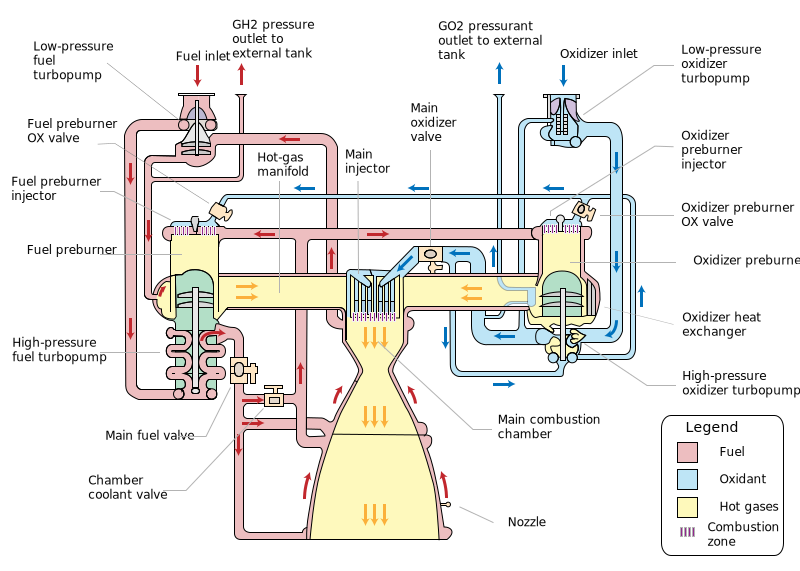
\includegraphics[width=.75\textwidth]{ssme_ciclo}
	\caption{A functional diagram showing the flow of propellant through an RS-25 engine.}
	\label{fig:ssme_cycle}
\end{figure}
\Cref{fig:ssme_cycle} is missing some components, such as the pogo oscillation suppression system accumulator, mounted before the oxidizer \acrshort{hptp}. However this goes beyond the scope of our analysis and will be disregarded.
 \end{document}
